\chapter{Three-Dimensional Potential Flows}
\begin{equation}
\left.
\begin{aligned}
\text{Incompressible}&\colon\nabla\cdot\mathbf{v}=0\\
\text{Irrotational}&\colon\nabla\times\mathbf{v}=0
\end{aligned}
\right\}
\Longrightarrow\nabla^2\Phi = 0,\mathbf{v}=\nabla\Phi
\end{equation}
\section{General Solution to 3D Axisymmetric Potential Flows}
\subsection{Governing Equations}
\begin{equation}
\nabla^2\Phi = 0
\label{eq: 7-1-1}
\end{equation}
Since axisymmetric, adopt spherical coordinate ($r,\theta,\varphi$)
\begin{figure}[H]
\centering
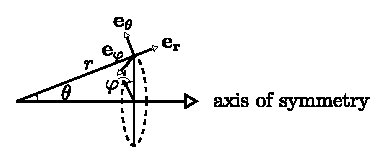
\includegraphics[scale=1.8]{figure/chapter7/7-1-1.eps}
%\caption{\label{fig:blue_rectangle} Rectangle}
\end{figure}
\begin{align*}
\nabla^2\Phi=0, &&(\frac{\partial}{\partial\varphi} = 0)
\end{align*}

\begin{equation}
\frac{1}{r^2}\frac{\partial}{\partial r}\left(r^2\frac{\partial\Phi}{\partial r}\right) + \frac{1}{r^2\sin\theta}\frac{\partial}{\partial\theta}\left(\sin\theta\frac{\partial\Phi}{\partial\theta}\right) = 0
\label{eq: 7-1-2}
\end{equation}
(Laplace equation)
\begin{itemize}
\item Stream function- Stokes' stream function\\
Recall vector potential in spherical coordinates
\[
\boldsymbol{\Psi} = \mathbf{e_\varphi}\frac{1}{r\sin\theta}\underbrace{\psi}_{
\begin{subarray}{c}
  \text{Stokes'}\\
  \text{stream function}
\end{subarray}
}
\]
where
\begin{subequations}
\label{eq: 7-1-3}
\begin{align}
v_r = \frac{1}{r^2\sin\theta}\frac{\partial\psi}{\partial\theta} \label{eq: 7-1-3a}\\
v_\theta = -\frac{1}{r\sin\theta}\frac{\partial\psi}{\partial r}\label{eq: 7-1-3b}
\end{align}
\end{subequations}
and governing equation for $\boldsymbol{\Psi}$
\begin{align*}
\nabla^2\boldsymbol{\Psi} = 0&&\text{i.e.}&&\nabla^2\left(\mathbf{e}_\varphi\frac{1}{r\sin\theta}\psi\right)=0
\end{align*}
spelling out
\begin{equation}
\Longrightarrow
\underbrace{\frac{\partial^2\psi}{\partial r^2}+\frac{\sin\theta}{r^2}\frac{\partial}{\partial\theta}\left(\frac{1}{\sin\theta}\frac{\partial\psi}{\partial\theta}\right) = 0}_{\text{Not Laplace equation}}
\label{eq: 7-1-4}
\end{equation}
\end{itemize}
\subsection{General Solution to the Potential Equation for Axisymmetric Flows}
\[
\frac{1}{r^2}\frac{\partial}{\partial r}\left(r^2\frac{\partial\Phi}{\partial r}\right) + \frac{1}{r^2\sin\theta}\frac{\partial}{\partial\theta}\left(\sin\theta\frac{\partial\Phi}{\partial\theta}\right) = 0
\]
Use separation of variables
\begin{equation}
\text{Let }\Phi(r,\theta)=f(r)g(\theta)\label{eq: 7-1-5}
\end{equation}
Substitute into \eqref{eq: 7-1-2} 
\[
\frac{1}{f}\frac{d}{dr}\left(r^2\frac{df}{dr}\right) = -\frac{1}{g\sin\theta}\frac{d}{d\theta}\left(\sin\theta\frac{dg}{d\theta}\right)=\text{ constant }\equiv\lambda
\]
For $f(r)\colon$
\begin{equation}
\frac{d}{dr}\left(r^2\frac{df}{dr}\right)-\lambda  f = 0\label{eq: 7-1-6}
\end{equation}
Let $f(r)=Ar^\alpha$ subs into \eqref{eq: 7-1-6}
\[
\alpha\left(\alpha+1\right)Ar^\alpha - \lambda Ar^\alpha = 0\Longrightarrow\alpha\left(\alpha+1\right) -\lambda = 0
\]
\begin{subequations}
\label{eq: 7-1-7}
\begin{align}
\alpha_1 = \frac{-1+\sqrt{1+4\lambda}}{2} \label{eq: 7-1-7a}\\
\alpha_2 = \frac{-1-\sqrt{1+4\lambda}}{2}\label{eq: 7-1-7b}
\end{align}
\end{subequations}
\begin{equation}
\Longrightarrow f(r) = A_1r^{\alpha_1} + A_2r^{\alpha_2}
\label{eq: 7-1-8}
\end{equation}
For $g(\theta)\colon$
\begin{equation}
\frac{1}{\sin\theta}\frac{d}{d\theta}\left(\sin\theta\frac{dg}{d\theta}\right) + \lambda g = 0
\label{eq: 7-1-9}
\end{equation}
Let $x=\cos\theta$
\begin{equation}
\Longrightarrow \frac{d}{dx}\left[\left(1-x^2\right)\frac{dg}{dx}\right] + \lambda g = 0,\phantom{-}-1\leq x\leq 1
\end{equation}
This is a Legendre differential equation\\
Solution is Legendre polynomials with $\lambda = n\left(n+1\right)$, $n=0,1,2,\cdots$ (eigenvalues)\\
\[
n=0\Longrightarrow P_0(x)=1
\]
\[
n=1\Longrightarrow P_1(x)=x=\cos\theta
\]
\begin{align*}
n&=2\\
\Longrightarrow 
P_2(x)&=\frac{1}{2}\left(3x^2-1\right) = \frac{1}{2}\left(3\cos^2\theta -1\right) = \frac{1}{4}\left(3\cos 2\theta +1\right)
\end{align*}
\begin{align*}
n&=2\\
\Longrightarrow 
P_2(x)&=\frac{1}{2}\left(3x^2-1\right) = \frac{1}{2}\left(3\cos^2\theta -1\right)\\ 
&= \frac{1}{4}\left(3\cos 2\theta +1\right)
\end{align*}
\begin{align*}
n&=3\\
\Longrightarrow 
P_3(x)&=\frac{1}{2}\left(5x^3-3x\right) = \frac{1}{2}\left(5\cos^3\theta -3\cos\theta\right)\\ 
&= \frac{1}{8}\left(5\cos 3\theta +3\cos\theta\right)
\end{align*}
hence 
\begin{align*}
g(x) = \sum_{n=0}^\infty a_n P_n(x)&&\text{or}&&g(\theta) = \sum_{n=0}^\infty a_n P_n(\cos\theta)
\end{align*}
Combine $f(r),g(\theta)$, since $\lambda= n\left(n+1\right)$
\[
\eqref{eq: 7-1-7}\Longrightarrow
\left\{
\begin{aligned}
\alpha_1 &= n \\
\alpha_2 &= -\left(n+1\right)
\end{aligned}
\right.
\]
i.e.
\[
f(r) = A_1r^n + \frac{A_2}{r^{n+1}}
\]
so
\begin{equation}
\Phi = f(r)g(\theta) = \boxed{\sum_{n=0}^\infty\left(A_nr^n + \frac{B_n}{r^{n+1}}\right)P_n(\cos\theta)}
\label{eq: 7-1-15}
\end{equation}
\section{Some Elementary 3D Potential Flows}
\begin{equation}
\Phi(r,\theta) = \sum_{n=0}^\infty\left(A_nr^n + \frac{B_n}{r^{n+1}}\right)P_n(\cos\theta)
\label{eq: 7-2-1}
\end{equation}
\begin{itemize}
\item Uniform flow\\
In \eqref{eq: 7-2-1}, take $B_n = 0$ for all $n's$ and $P_1(\cos\theta)=\cos\theta$
\begin{align*}
A_n = U\text{ for }n=1 && A_n= 0\text{ for }n\neq 1
\end{align*}
$\therefore$ \eqref{eq: 7-2-1} gives $\Longrightarrow$
\begin{equation}
\Phi(r,\theta) = Ur\cos\theta
\label{eq: 7-2-2}
\end{equation}
%----------------------
\begin{minipage}{0.6\textwidth}
\begin{subequations}
\label{eq: 7-2-3}
\begin{align}[left = \empheqlbrace\,]
v_r&=\frac{\partial\Phi}{\partial r} = U\cos\theta \label{eq: 7-2-3a} \\
v_\theta&=\frac{1}{r}\frac{\partial\Phi}{\partial \theta} = -U\sin\theta  \label{eq: 7-2-3b}
\end{align}
\end{subequations}
\end{minipage} \hfill
\begin{minipage}{0.5\textwidth}
\begin{tikzpicture}
\coordinate (O) at (0,0);
\coordinate (x) at (4,0);
\coordinate (p) at (3,2);
\fill[color=black] (p) circle[radius=2pt] node[below right]{$(r,\theta)$};
\draw [arrows = {-Latex[color=black, fill=white, length=3mm]}] (O) -- (x) node [at end, right] {$x$};
\draw [-] (O) -- (p) node [pos=0.7, anchor=east] {$r$};
\draw [-{Latex[length=2mm]}, rotate=0] (p) -- ($(p)+(0.6,0.4)$) node [above right] {$v_r=U\cos\theta$} ;
\draw [-{Latex[length=2mm]}, rotate=0] (p) -- ($(p)+(-0.4,0.6)$) node [above left] {$v_r=U\cos\theta$} ;
\draw[->] (-3,1) -- (-2,1) node[pos=0.5, anchor=south]{$U$};
\draw[->] (-3,0) -- (-2,0);
\draw[->] (-3,-1) -- (-2,-1);
\draw pic["$\theta$", draw=black, text=black, -{Latex[length=2mm]}, angle eccentricity=1.4, angle radius=1.0cm] {angle=x--O--p};
\end{tikzpicture}
\end{minipage}\\
%----------------------
\begin{exercise}{Show that the Stokes' stream function for uniform flow is}
\begin{equation}
\psi(r,\theta) = \frac{1}{2}Ur^2\sin^2\theta
\label{eq: 7-2-4}
\end{equation}
using
\begin{align*}
v_r = \frac{1}{r^2\sin\theta}\frac{\partial\psi}{\partial\theta}, &&v_\theta = -\frac{1}{r\sin\theta}\frac{\partial\psi}{\partial r}
\end{align*}
\end{exercise}
\item Point source/sink\\
In \eqref{eq: 7-2-1}, take $A_n = 0$ for all $n's$ and $P_0(\cos\theta)=1$
\begin{align*}
B_n = B_0\text{ for }n=0 && B_n= 0\text{ for }n\neq 0
\end{align*}
$\therefore$ \eqref{eq: 7-2-1} gives $\Longrightarrow$
\begin{equation}
\Phi(r,\theta) = \frac{B_0}{r}
\label{eq: 7-2-5}
\end{equation}
Velocity components are
\begin{subequations}
\label{eq: 7-2-6}
\begin{align}[left = \empheqlbrace\,]
v_r&=\frac{\partial\Phi}{\partial r} = -\frac{B}{r^2} \label{eq: 7-2-6a} \\
v_\theta&=\frac{1}{r}\frac{\partial\Phi}{\partial \theta} = 0  \label{eq: 7-2-6b}
\end{align}
\end{subequations}
volume flow rate is 
\begin{align*}
Q
&= \oiint_S\mathbf{v}\cdot\mathbf{n}dS = \int_{\varphi = 0}^\pi d\varphi\int_{\theta=0}^\pi\left(-\frac{B_0}{r^2}\right)r^2\sin\theta d\theta \\
&= -4\pi B_0
\end{align*}
\begin{equation}
\therefore\Phi = \frac{B_0}{r} = -\frac{Q}{4\pi r}
\label{eq: 7-2-7}
\end{equation}
where 
\begin{alignat*}{4}
& B_0\colon     \quad && \text{"$-$"}\Longrightarrow \quad && Q\colon \quad && \text{"$+$"}\Longrightarrow\text{source}\\
& B_0\colon     \quad && \text{"$+$"}\Longrightarrow \quad && Q\colon \quad && \text{"$-$"}\Longrightarrow\text{sink}
\end{alignat*}
\begin{exercise}{Show that the Stokes' stream function for source/sink is}
\begin{align}
\psi(r,\theta) 
&= \frac{1}{2}Ur^2\sin^2\theta \nonumber \\
&= -\frac{Q}{4\pi}\left(1+\cos\theta\right) \label{eq: 7-2-8}
\end{align}
\end{exercise}
\item Doublet
\begin{center}
\begin{tikzpicture}
\coordinate (O) at (0,0);
\coordinate (x) at (4,0);
\coordinate (-x) at (-4,0);
\coordinate (P) at (3,2);
\coordinate (-Q) at (2,0);
\coordinate (Q) at (-2,0);
\fill[color=black] (O) circle[radius=2pt] node[below]{$O$};
\fill[color=black] (Q) circle[radius=2pt] node[below]{$Q$};
\fill[color=black] (-Q) circle[radius=2pt] node[below]{$-Q$};
\fill[color=black] (P) circle[radius=2pt] node[above right]{$P$};
\draw [-] (O) -- (P) node [pos=0.5, anchor=east] {$r$};
\draw [-] (Q) -- (P) node [pos=0.5, anchor=east] {$r_1$};
\draw [-] (-Q) -- (P) node [pos=0.5, anchor=east] {$r_2$};
\draw [arrows = {-Latex[color=black, fill=white, length=3mm]}] (-x) -- (x) node [at end, right] {$x$};
\draw[-](Q) -- (O) node [pos=0.5, anchor=south] {$\epsilon$};
\draw[-](O) -- (-Q) node [pos=0.5, anchor=south] {$\epsilon$};
\draw pic["$\theta$", draw=black, text=black, -{Latex[length=2mm]}, angle eccentricity=1.2, angle radius=1.5cm] {angle=-Q--O--P};
\end{tikzpicture}
\end{center}
\begin{align}
\text{at }P\colon &&\Phi(r,\theta) = -\frac{Q}{4\pi r_1} + \frac{Q}{4\pi r_2}
\label{eq: 7-2-9}
\end{align}
but
\begin{align*}
r_1^2
&= r^2 + \epsilon^2 - 2\epsilon r\cos(\pi-\theta) \\
&= r^2 + \epsilon^2 + 2\epsilon r\cos\theta \\
&= r^2\left[1 + \left(\frac{\epsilon}{r}\right)^2 + \left(\frac{2\epsilon}{r}\right)\cos\theta\right]
\end{align*}
\[
\therefore\frac{1}{r_1^2}\approx\frac{1}{r^2}\left[1-\frac{2\epsilon}{r}\cos\theta + \mathcal{O}(\frac{\epsilon}{r})^2\right]
\]
Similarly
\[
\therefore\frac{1}{r_2^2}\approx\frac{1}{r^2}\left[1+\frac{2\epsilon}{r}\cos\theta + \mathcal{O}(\frac{\epsilon}{r})^2\right]
\]
\begin{align*}
\therefore\Phi(r,\theta)
&= -\frac{Q}{4\pi}\left(\frac{1}{r_1}-\frac{1}{r_2}\right) \\
&\approx -\frac{Q}{4\pi}\frac{1}{r}\left[\sqrt{1-\frac{2\epsilon}{r}\cos\theta} - \sqrt{1+\frac{2\epsilon}{r}\cos\theta}\right] \\
&\approx -\frac{Q}{4\pi r}\left[\left(1-\frac{\epsilon}{r}\cos\theta\right) - \left(1+\frac{\epsilon}{r}\cos\theta\right)\right] \\
&= \frac{2\epsilon Q}{4\pi r^2}\cos\theta
\end{align*}
let $\epsilon\to 0$ and $Q\to\infty$, such that $2\epsilon Q\to \mu$, then
\begin{equation}
\Phi(r,\theta) = \frac{\mu\cos\theta}{4\pi r^2}
\label{eq: 7-2-10}
\end{equation}
where $\mu$ is strength of the doublet\\

velocity components are
\begin{subequations}
\label{eq: 7-2-6}
\begin{align}[left = \empheqlbrace\,]
v_r&=\frac{\partial\Phi}{\partial r} = -\frac{\mu}{2\pi r^3}\cos\theta \label{eq: 7-2-6a} \\
v_\theta&=\frac{1}{r}\frac{\partial\Phi}{\partial \theta} = -\frac{\mu}{4\pi r^3}\sin\theta  \label{eq: 7-2-6b}
\end{align}
\end{subequations}
\begin{exercise}{Show that the Stokes' stream function for doublet is}
\begin{align}
\psi(r,\theta) 
= -\frac{\mu}{4\pi r}\sin^2\theta \label{eq: 7-2-8}
\end{align}
\end{exercise}
\end{itemize}
\section{Flows Generated by Superposition}
\subsection{Rankine Bodies}
\begin{center}
\begin{tikzpicture}
\coordinate (O) at (0,0);
\coordinate (x) at (4,0);
\coordinate (-x) at (-4,0);
\coordinate (P) at (3,2);
\coordinate (-Q) at (2,0);
\coordinate (QQ) at (2,0);
\coordinate (Q) at (-2,0);
\fill[color=black] (O) circle[radius=2pt] node[below]{$O$};
\fill[color=black] (Q) circle[radius=2pt] node[below]{$Q$};
\fill[color=black] (-Q) circle[radius=2pt] node[below]{$-Q$};
\fill[color=black] (P) circle[radius=2pt] node[above right]{$P(r,\theta)$};
\draw [-] (O) -- (P) node [pos=0.5, anchor=east] {$r$};
\draw [-] (Q) -- (P) node [pos=0.5, anchor=east] {$r_1$};
\draw [-] (-Q) -- (P) node [pos=0.5, anchor=east] {$r_2$};
\draw [arrows = {-Latex[color=black, fill=white, length=3mm]}] (Q) -- (x) node [at end, right] {$x$};
\draw[-](Q) -- (O) node [pos=0.5, anchor=north] {$l$};
\draw[-](O) -- (-Q) node [pos=0.5, anchor=north] {$l$};
\draw pic["$\theta$", draw=black, text=black, -{Latex[length=2mm]}, angle eccentricity=1.2, angle radius=1.5cm] {angle=-Q--O--P};
\draw pic["$\theta_1$", draw=black, text=black, -{Latex[length=2mm]}, angle eccentricity=1.2, angle radius=1.5cm] {angle=O--Q--P};
\draw pic["$\theta_2$", draw=black, text=black, -{Latex[length=2mm]}, angle eccentricity=1.2, angle radius=1.5cm] {angle=x--QQ--P};
\draw[->] (-4,1) -- (-3,1) node[pos=0.5, anchor=south]{$U$};
\draw[->] (-4,0) -- (-3,0);
\draw[->] (-4,-1) -- (-3,-1);
\end{tikzpicture}
\end{center}
\begin{equation}
\Phi = Ur\cos\theta - \frac{Q}{4\pi r_1} + \frac{Q}{4\pi r_2},\phantom{-}Q>0
\label{eq: 7-3-1}
\end{equation}
Stream function is
\begin{equation}
\psi = \frac{1}{2}Ur^2\sin^2\theta - \frac{Q}{4\pi}\cos\theta_1 + \frac{Q}{4\pi}\cos\theta_2
\end{equation}
\begin{exercise}{Show that}
\[
\left\{
\begin{aligned}
\left(L^2-l^2\right)^2-\frac{Ql}{\pi U}L &= 0\\
h^2\sqrt{h^2+l^2} - \frac{Ql}{\pi U} = 0
\end{aligned}
\right.
\]
\end{exercise}
\subsection{Uniform Flow Past a sphere}
Stokes' stream function is
\[
\psi = \frac{U}{2}r^2\sin^2\theta - \frac{\mu}{4\pi r}\sin^2\theta
\]
require $\psi = 0$ at $r=a\Longrightarrow \mu = 4\pi Ua^3$ , i.e.
\begin{equation}
\psi = \frac{U}{2}\left(r^2-\frac{a^3}{r}\right)\sin^2\theta
\label{eq: 7-3-8}
\end{equation}
\begin{exercise}{Show that}
\begin{equation}
\Phi = U\left(r + \frac{a^3}{2r^2}\right)\cos\theta
\label{eq: 7-3-9}
\end{equation}
\end{exercise}
velocity components
\begin{subequations}
\label{eq: 7-3-10}
\begin{align}[left = \empheqlbrace\,]
v_r&=\frac{\partial\Phi}{\partial r} = U\left(1-\frac{a^3}{r^3} \right)\cos\theta\label{eq: 7-3-10a} \\
v_\theta&=\frac{1}{r}\frac{\partial\Phi}{\partial \theta} = -U\left(1+\frac{a^3}{2r^3}\right)\sin\theta  \label{eq: 7-3-10b}
\end{align}
\end{subequations}
velocities on the sphere
\[
\left\{
\begin{aligned}
v_r &= 0\\
v_\theta &= -\frac{3}{2}U\sin\theta
\end{aligned}
\right.
\]
<cf> 2D cylinder
\[
\left\{
\begin{aligned}
v_r &= 0\\
v_\theta &= -2U\sin\theta
\end{aligned}
\right.
\]